\documentclass[notitlepage,twocolumn, 12pt]{report}
\usepackage{mypackagesv2}
\usepackage{float}
\usepackage{atbegshi}% http://ctan.org/pkg/atbegshi % lazy way to remove extra page
\AtBeginDocument{\AtBeginShipoutNext{\AtBeginShipoutDiscard}}
\setlength{\belowcaptionskip}{-10pt}
\tolerance=1
\emergencystretch=\maxdimen
\hyphenpenalty=10000
\hbadness=10000


\title{Testing a Model to Predict the Motion of a Pendulum} % bad title fix
\author{Pranav Upreti | PHY 180 Lab 1}

\begin{document}
    \maketitle
    \setcounter{page}{1}
    \begin{abstract}
    This experiment tested Brian Wilson's model to predict the motion of a pendulum. A pendulum was constructed from household materials and its Q factor was measured to be 270 $\pm$ 20. The experimental results indicate that Wilson's model is most accurate for small release angles, but drag and friction forces should be considered to improve the model. 
    \end{abstract}
    \section{Introduction}
    An accurate model for the periodic motions, such as in a pendulum, is useful because of how common periodic motions are in nature. If we consider the simplest case of periodic motion, coined simple harmonic motion, a particle oscillates indefinitely about some equilibrium position. The position of the particle can be modelled as a sinusoidal function, $x(t) = A\cos(\omega t)$ where $A$ is the greatest displacement away from equilibrium, and $\omega$ is related to the period of oscillations. This makes sense intuitively, since sinusoidal functions are periodic, and it is well known how to derive this result mathematically so a derivation is omitted. 

    This model assumes that no energy is lost in an oscillating system. But in reality, oscillating systems slow down and stop. This is due to \textit{non-conservative} forces which dissipate energy to surroundings. For this experiment, we will assume that drag forces are negligible because the pendulum mass (a 500 mL water bottle) has a small cross-section and travels at low speeds. Instead, we define a damping force, $-b \diff{x}{t}$ proportional to the velocity of the pendulum mass (OpenStax, n.d.):
    \begin{align*}
        m \diff[2]{x}{t} &= - b \diff{x}{t} - kx \\
        \intertext{where $b$ is some constant, and $k$ is the spring constant of the rope. After rearrange we see that}
        0 &= m \diff[2]{x}{t} + b \diff{x}{t} + kx   \\
    \intertext{this is a linear differential equation (OpenStax, n.d.) whose solution is} 
        x(t) &= A_0e^{\nicefrac{-bt}{2m}}\cos(\omega t + \phi)
    \end{align*} 
    Wilson's model is the same, except it predicts angle with time instead of position. As well, it introduces a constant $\nicefrac{1}{\tau} = \nicefrac{b}{2m}$ and uses $\omega = \nicefrac{2 \pi}{T}$ to get the equation:
    \begin{equation}\label{eq:1}
        \theta(t) = \theta_0 e^{-\nicefrac{t}{\tau}}\cos(\nicefrac{2\pi}{T} + \phi)
    \end{equation}
    This equation predicts exponential decay in the amplitude of $\theta$-$t$ graph. We can "measure" this decay by calculating the \textit{Q factor} of the pendulum: $Q = \nicefrac{\pi \tau}{T}$. $Q$ can be calculated by first finding $\tau$ using experimental data, and by measuring the number of oscillations until the amplitude of oscillation is $\theta_0e^{-\pi}$. Both methods will be used to calculate $Q$. 
    
    % viscous force, air drag, and damped harmonic oscillations
    % assumptions in the model and predicted result
    \section{Method}
    An 85.0 $\pm$ 0.05 cm jute twine string with mass < 10.0 $\pm$ 0.1 g was tied from one end to a 500 mL plastic water bottle filled with water to a mass of 500 $\pm$ 0.1 g. The other end of the jute twine was tied to a nail 100.0 $\pm$ 0.05 cm above the ground. The jute twine was tied tightly enough so that no  slipping was observed when the mass swung. To record the motion of the pendulum, a smartphone camera was positioned 120.0 $\pm$ 0.05 cm away from the pendulum setup. The camera video feed was saved and inputted into an application called \textit{Tracker} which automatically tracks the horizontal and vertical position of the pendulum with time. To calibrate the distance scale in the tracker application, a piece of 28 $\pm$ 0.05 cm paper was placed on the plane of the pendulum motion. The origin of the coordinate system was the center of the video frame. Black tape was placed on the water bottle to help the AutoTracker distinguish the water bottle from the light-coloured background. 
    Data from \textit{Tracker} was processed and graphed using a script provided by Wilson, with modifications to plot peak amplitudes of the graph (see Appendix).
    The mass was swung from 1.40 $\pm$ 0.01 rad to -1.40 $\pm$ 0.01 rad in increments of 0.35 $\pm$ 0.01 rad. The Tracker application plots a position-time graph, and the period was measured from this graph. This data is included in the Appendix and was processed to determine the relationship between release angle. The same data was used to determine the Q factor of the pendulum
    \begin{figure}[H]
        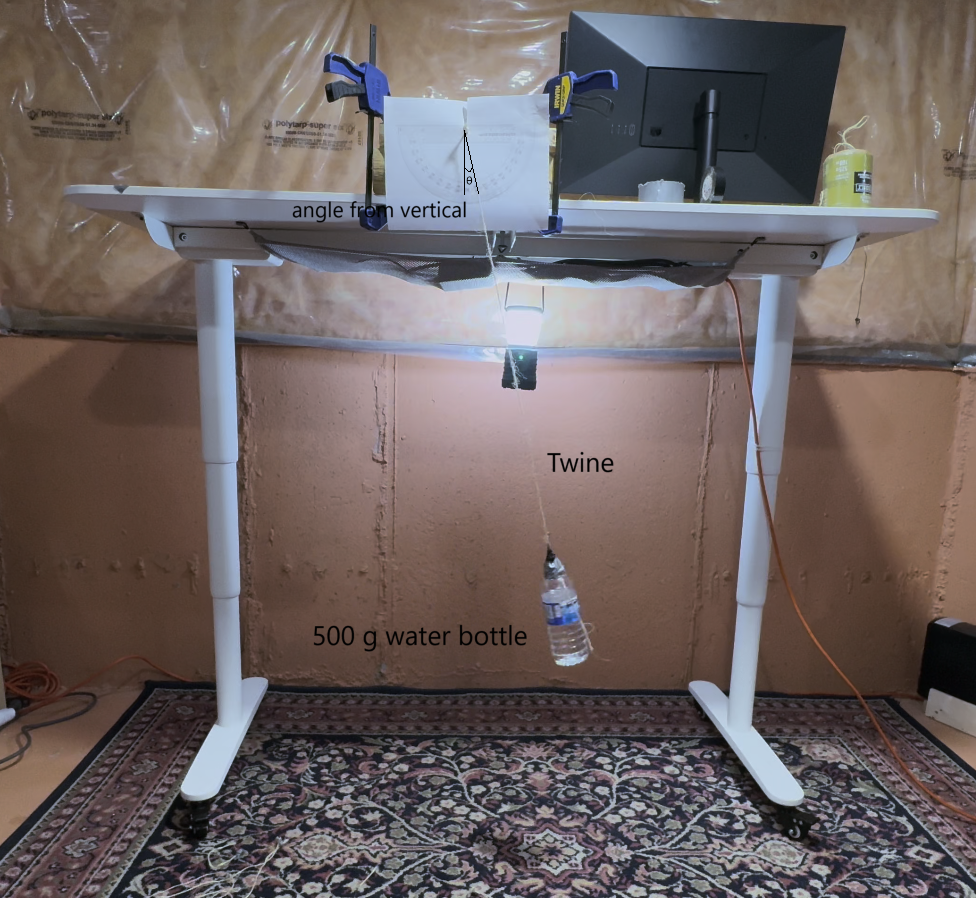
\includegraphics[width=\linewidth]{temp.png}
        \caption{The experimental setup}
    \end{figure}
    \section{Testing for Asymmetry}
    Wilson's model suggests that the period of the pendulum is independent to the pendulum's release angle (Equation 1). To test this, the pendulum mass was released from different angles measured from the vertical. The period was measured by counting ten periods and dividing by 10, to get the average period. 

    \begin{figure}[H]
        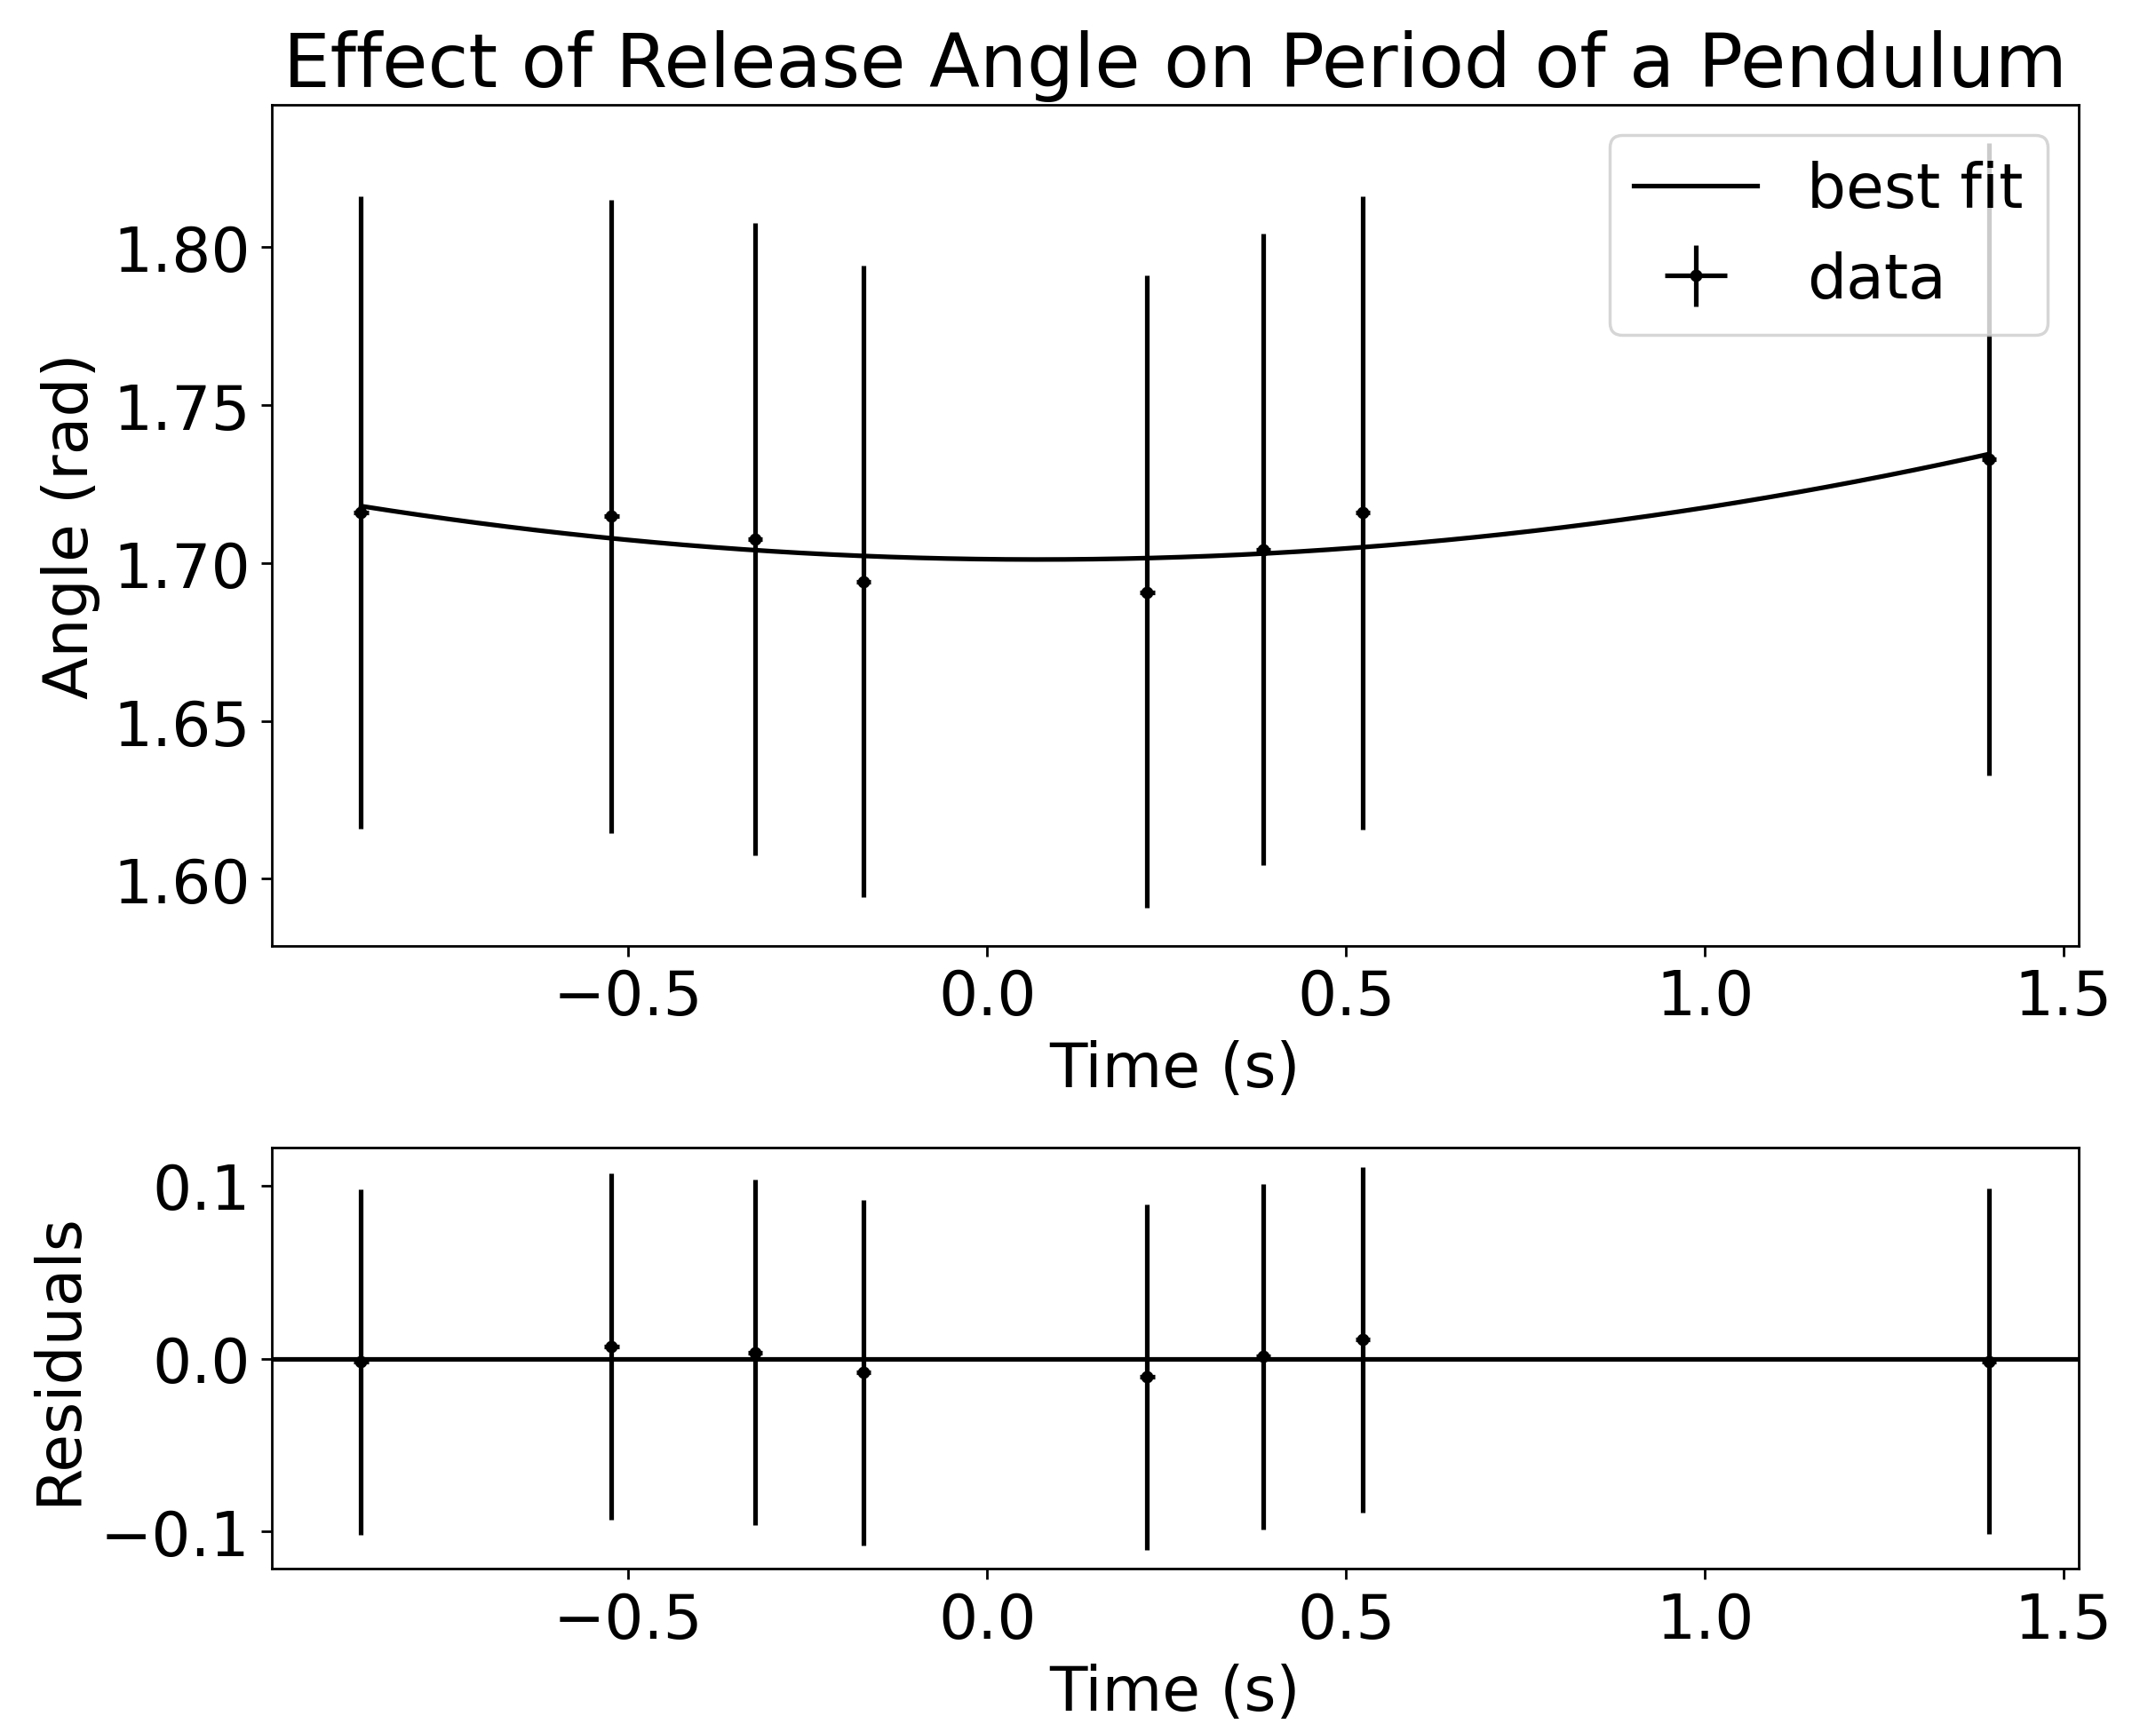
\includegraphics[width=\linewidth]{figure1.png}
        \caption{The period of the pendulum does depend on the release angle from the vertical. The line of best fit as calculated by the provided Python code (Wilson, 2024) was (0.02 $\pm$ - 0.07)$x^2$ -0.01 $\pm$ 0.06$x$ + 1.70 $\pm$ 0.05.}
    \end{figure}

    Figure 2 suggests that the pendulum depends on the release angle from the vertical. However, for the first and second order terms, the uncertainty is greater than its value. We deduce that the first and second order terms are experimentally zero, which indicates that the period of a pendulum is effectively constant. This deduction is more accurate for small pendulum release angles because quadratic functions scale quickly for larger $x$. 

    \section{Empirically determined Q factor}
    The horizontal position of the pendulum mass was recorded against time for each release angle (see Appendix).

    The Q factor can be measured based on the exponential decay of the amplitude with time. Hence, the amplitudes of the position-time graph were plotted and an exponential line of best fit was drawn. 

    Note: we determined empirically that the release angle of the pendulum is approximately independent to its period. This means the data from any trial can be used to determine the Q factor, and it should be approximately the same between trials. We found this to be true, when comparing the Q factor between trials at different angles. However, the Q factor was most consistent for small release angles, so the graph of 0.34 $\pm$ 0.01 rad was used below. 

    \begin{figure}[H]
        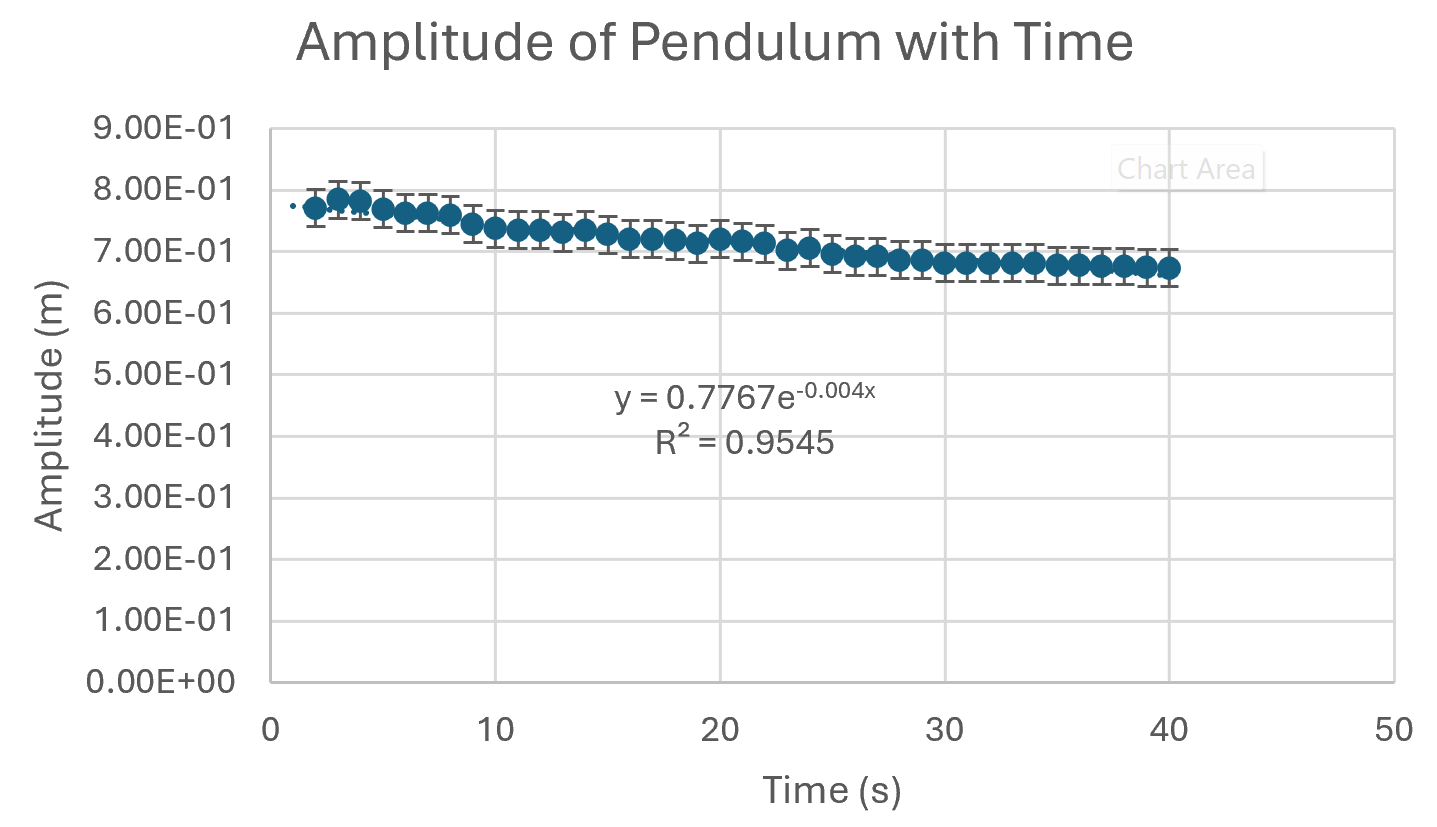
\includegraphics[width=\linewidth]{amplitudeTgraph.png}
        \caption{Graph of amplitude (m) vs time (s). Physlets Tracker was used to manually plot the location of the pendulum apexes with respect to time when the pendulum was at different angles from the vertical (-1.39, 1.39)$\pm$ 0.01 rad. The graph suggests that $\tau$ = 700 $\pm$ 100, and was calculated with the provided python script created by Wilson. Horizontal error bars are too small to be seen, and was calculated to be the length of one frame (because amplitudes were found by scrubbing 2 frames). The vertical error bars were calculated as half the width of the bottle cap}
    \end{figure}

    We can use the empirically determined value for $\tau$ to calculate the Q factor. Recall that $Q = \nicefrac{\tau \pi}{T} = \nicefrac{700\pi}{T} \pm (\nicefrac{100}{700})\times 100\% = 1300 \pm 200 s^{-1}$. A Q factor of 270 $\pm$ 20 was also determined by counting the number of periods until the amplitude is $e^{-pi}=4\%$ of its original amplitude. Since the Q factor is proportional to time, its percentage uncertainty matches the uncertainty in time.
    
    The two methods of calculating the Q factor give significantly different results, even while considering their uncertainties. For this report, we chose the Q factor with the counting method. This is because using an equation to derive Q assumes Wilson's model is correct, but the counting method does not make this assumption. 
    \section{Uncertainties}
    The uncertainty in measuring equipment was larger than the uncertainty predicted by calculating the standard deviation between several trials. Hence, measurement equipment uncertainty is largely propagated through this report. The measurement equipment included measuring tape ($\pm$ 0.05 cm), a digital scale ($\pm$ 0.1 g), and a protractor ($\pm$ 0.05$^\circ$). 
    These uncertainties are too conservative though. In Figure 2, all the residuals pass through 0 which suggests that the error bars are too large. Using more precise equipment will be helpful to draw different conclusions from data with smaller error bars. 
    The largest source of error is the position of the pendulum mass, which was tracked in software. We chose this uncertainty as half the width of the mass, which was propagated by the provided Python script, along with all uncertainties (see Appendix for code). This uncertainty can be reduced by making tracking more accurate, so we can be confident it tracks the pendulum motion accurately. This is discussed in the conclusion. 
    \section{Conclusion}
    In this experiment, we constructed a pendulum with household materials with the goal of testing Wilson's model of pendulum motion. The model predicts an independence of release angle from the pendulum period, and the data supports this for small release angles; for large release angles an increase in period was evident (Figure 2). Further, we calculated the Q factor of the pendulum to be 270 $\pm$ 20.
    \subsection{Discussion}
    The Q factor was calculated it two ways from the data in Figure 3. The counting method gave Q = 270 $\pm$ 20 and the equation method gave Q = 1300 $\pm$ 200. We chose Q = 270 $\pm$ 20 because it does not assume Wilson's model to be correct. However, there may be problems with the experiment. For instance, we may have wrongly considered parallax error to be insignificant because it would not impact trends in collected data provided the error is consistent between trials. There were also issues with Autotracker in Tracker skipping frames and beginning to track the incorrect pixels. We did retrack those frames, but it suggests the current setup is suboptimal for software based tracking. Next time, reflective tape can be placed on the bottle so pixel tracking is more consistent. 
    It may also be that Wilson's model is incorrect. Considering that the counting method was significantly smaller than the equation method suggests that Wilson's model did not consider all damping forces. Namely, there may have been non-negligible friction forces between the string and the nail it was tied to, or significant drag forces. This makes sense because the model should always overpredict Q since it predicts fewer damping forces. Next time, numerical modelling can be used to predict the drag forces on the mass.

    \section{Citations}
    \begin{figure}[H]
        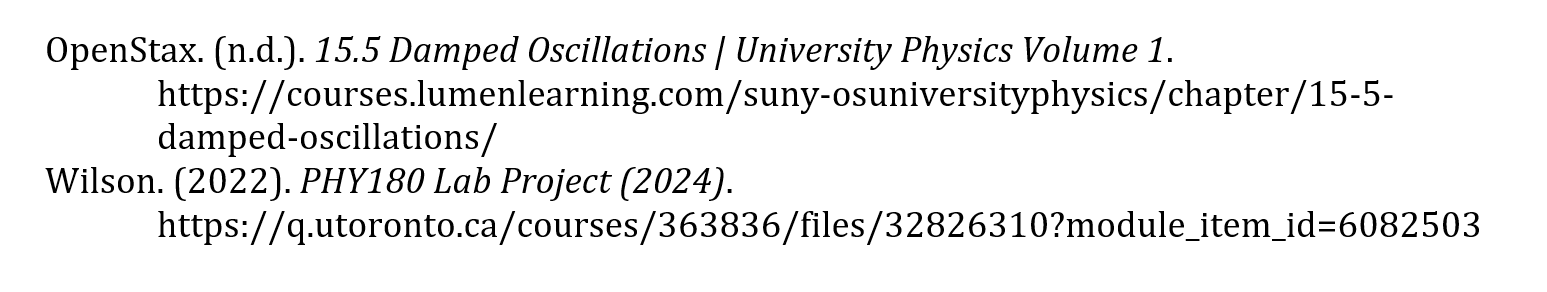
\includegraphics[width=\linewidth]{citations.png}
    \end{figure}

    \section{Appendix}
    All data and code is stored \href{https://github.com/PRU1/PHY180-pendulum-project}{here}.



    \textit{NOTE: this document is under 3 pages without the title, abstract, and appendix. I wanted to include an introduction to reduce my workload later on, when we write the full report.}

\end{document}